%%%%%%%%%%%%%%%%%%%%%%%%%%%%%%%%%%%%%%%%%%%%%%%%%%%%%%%%%%%%%%%%%%%%%%%%%%%%%%%%
%2345678901234567890123456789012345678901234567890123456789012345678901234567890
%        1         2         3         4         5         6         7         8
\documentclass[letterpaper, 10 pt, conference]{ieeeconf}  % Comment this line out
                                                          % if you need a4paper
%\documentclass[a4paper, 10pt, conference]{ieeeconf}      % Use this line for a4

\usepackage{float}
                                                          % paper
% uso paquete bookmark para tener bien los outlines.
\usepackage{bookmark}

% Configuro el idioma.
\usepackage[utf8]{inputenc} % Importante para mantener acentos.
\usepackage[spanish, activeacute]{babel} % Requiere: texlive-lang-spanish. Por primera vez hay que ejecutar: texconfig init> log

% Paquete para poder usar acentos en $$.
\usepackage{mathtools}
%\setmathfont{XITS math}

% Para los diagramas de flujo
\usepackage{tikz}
\usetikzlibrary{shapes.geometric, arrows}

% Elementos del diagrama
\tikzstyle{startstop} = [rectangle, rounded corners, 
minimum width=6em, 
minimum height=2em,
text centered, 
draw=black, 
fill=red!30]

\tikzstyle{io} = [trapezium, 
trapezium stretches=true, % A later addition
trapezium left angle=70, 
trapezium right angle=110, 
minimum width=6em, 
minimum height=2em, text centered, 
draw=black, fill=blue!30]

\tikzstyle{block} = [rectangle, 
minimum width=8em, 
minimum height=3em, 
text centered, 
text width=7.5em, 
draw=black, 
fill=white!30]

\tikzstyle{def} = [rectangle, 
minimum width=14em, 
minimum height=3em, 
text centered, 
text width=12em, 
draw=black, 
fill=purple!30]

\tikzstyle{swap_proccess} = [rectangle, 
minimum width=8em, 
minimum height=2em, 
text centered, 
text width=8em, 
draw=black, 
fill=orange!30]

\tikzstyle{process} = [rectangle, 
minimum width=6em, 
minimum height=2em, 
text centered, 
text width=6em, 
draw=black, 
fill=orange!30]

\tikzstyle{decision} = [diamond, 
minimum width=6em, 
minimum height=6em, 
text centered, 
draw=black, 
fill=green!30]
\tikzstyle{arrow} = [thick,->,>=stealth]

\usepackage{siunitx}

% package to get \url
\usepackage{hyperref}
\hypersetup{
  colorlinks=true,
  linkcolor=magenta,
  filecolor=magenta,
  citecolor=magenta,      
  urlcolor=magenta,
}

% Graficos electrónicos
\usepackage[RPvoltages]{circuitikz}

\IEEEoverridecommandlockouts                              % This command is only
                                                          % needed if you want to
                                                          % use the \thanks command
\overrideIEEEmargins
% See the \addtolength command later in the file to balance the column lengths
% on the last page of the document

\usepackage{graphicx}
\usepackage{graphics}

% styling for matlab/octave code.
\usepackage{matlab-prettifier}
% Configuracion, con esto puede agregar ñ.
\lstset{
  literate={ñ}{{\~n}}1
}

\usepackage{listings}

% The following packages can be found on http:\\www.ctan.org
%\usepackage{graphics} % for pdf, bitmapped graphics files
%\usepackage{epsfig} % for postscript graphics files
%\usepackage{mathptmx} % assumes new font selection scheme installed
%\usepackage{times} % assumes new font selection scheme installed
\usepackage{amsmath} % assumes amsmath package installed
%\usepackage{amssymb}  % assumes amsmath package installed

\title{\LARGE \bf Entregable Trabajo Práctico N° 2}

\author{
  Tom\'as Vidal\\
  {\it Sistemas Operativos y Redes}\\
  {\it Facultad de Ingenier\'ia, UNLP, La Plata, Argentina.}\\
  {\it 14 de Octubre, 2024.}
}                                            % <-this % stops a space


% comienzo

% INTRO


% Figura
\newcommand{\image}[2] {
  \begin{figure}[H]
    \centering
    \includegraphics[width=0.43\textwidth]{./#1.png}
    \caption{#2}
    \label{fig:#1}
  \end{figure}
}

% Codigo
% \begin{lstlisting}[style=Matlab-editor]
% % el código va aca
% dispc("HELLO WORLD");
% \end{lstlisting}

\begin{document}
\maketitle
\thispagestyle{empty}
\pagestyle{empty}

\section{Problemas presentados}
\subsection{Problema 10}


\subsection{Problema 11}
Se debe crear un programa que pueda actuar de \textit{dos formas diferentes}, como: \textbf{proceso A} o \textbf{proceso B}. Ambos deben poder acceder a un \textit{bloque de memoria compartida}, para poder leer y escribir datos en común. Ambos procesos deben mantener una cierta sincronía, ya que uno no puede leer mientras el otro escribe y viceversa.

\section{Problema 11}
\subsection{Algorimo implementado}
En la figura \ref{fig:diag_flujo_p11} se muestra el flujo general del programa. El diagrama es \textit{abierto}, en sentido de que hay caminos en paralelo, esto se debe a que el programa tiene un comportamiento concurrente, ya que se registran manejadores de señales que esperan a ser llamados por \textbf{SIGUSR1} y \textbf{SIGTERM}.
\begin{figure*}[tb]
  \centering
  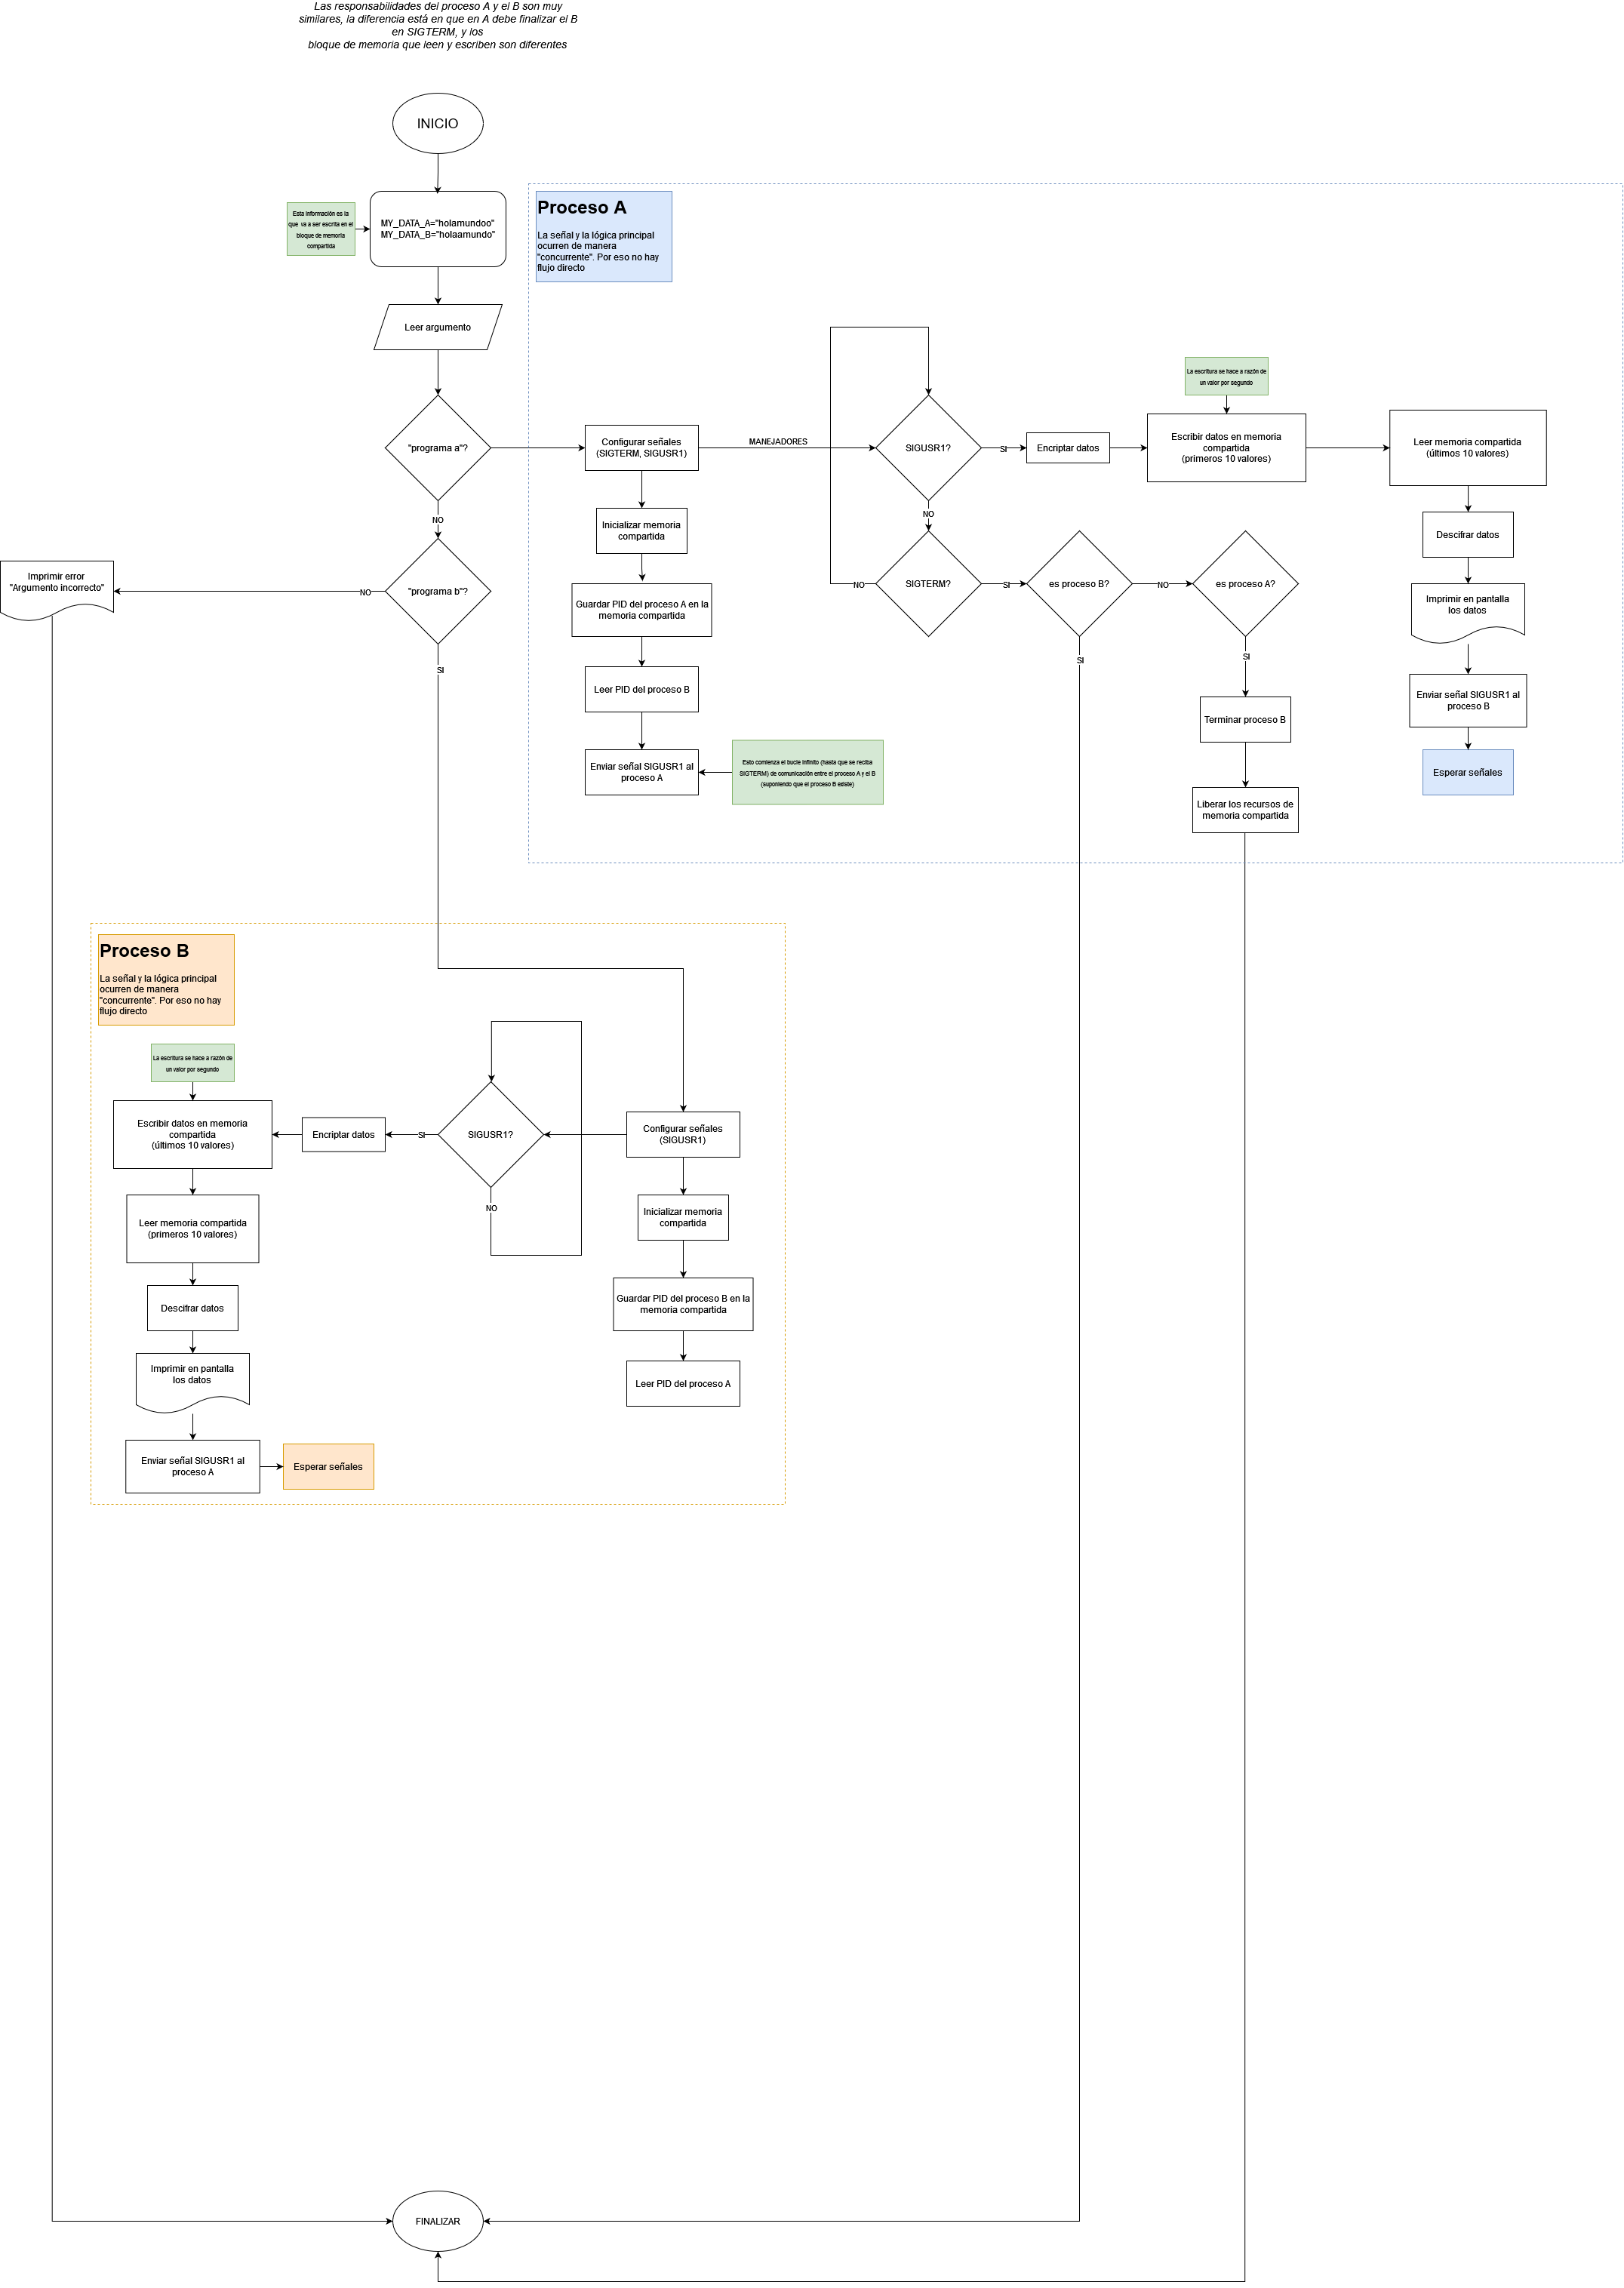
\includegraphics[width=\textwidth]{./diagrama_flujo_tp2.png}
  \caption{Diagrama de flujo del problema 11.}
  \label{fig:diag_flujo_p11}
\end{figure*}

\subsection{Funciones principales}
\begin{itemize}
  \item \textit{handle\_termination:} Manejador que se encarga de liberar los recursos y terminar ambos procesos.
  \item \textit{handle\_write\_read\_a:} Realiza la escritura y lectura acorde a las especificaciones del \textbf{proceso A}.
  \item \textit{handle\_write\_read\_b:} Realiza la escritura y lectura acorde a las especificaciones del \textbf{proceso B}.
  \item \textit{cypher:} Función de encriptación de datos.
  \item \textit{decypher:} Función de desencriptación de datos.
  \item \textit{setup\_shared\_memory:} Prepara la memoria compartida para ser usada.
  \item \textit{save\_pid\_to\_shared\_mem:} Guarda en la memoria compartida el PID del proceso actual (A o B).
  \item \textit{get\_pid\_from\_shared\_mem:} Obtiene el PID del proceso opuesto (A o B).
  \item \textit{destroy\_memory\_block:} Libera la memoria compartida.
\end{itemize}

\subsection{Explicación general del algorimo}
Se registran los manejadores para la señal \textbf{SIGUSR1} en ambos procesos; estos manejadores se encargan de la escritura y lectura correspondiente al proceso. Al incio el \textit{proceso A} se envía a sí mismo la señal \textbf{SIGUSR1}, de modo que si el \textit{proceso B} existe, comienza un bucle entre ambos procesos de lectura y escritura, ya que al finalizar estas operaciones, cada proceso envía al otro la misma señal \textbf{SIGUSR1}. \\
\textit{Para poder enviar señales entre ambos procesos, se emplea la memoria compartida para almacenar el PID correspondiente a ambos procesos, puesto que se guarda un arreglo de \textbf{int} y los PID son del mismo tipo.} \\
Al comienzo se definen los 20 \textbf{int}, que conforman las palabras 'holamundooholaamundo', encriptadas con las especificiones del problema (es decir son \textit{números del 0 al 26}, que representan las letras de la \textbf{a} a la \textbf{z}), posteriormente en la escritura de ambos procesos, se escriben estos datos nuevamente encriptados con la función provista $f(x)$, y cuando se leen se desencriptan con la función $f^{-1}(x)$

\section{Diagramas}
Se adjuntan junto al presente las figuras de los diagramas de flujo, para que el lector pueda analizarlas precisamente.


\end{document}
